% ----------------------------------------------------------------------
%  Pracovní úkoly
% ----------------------------------------------------------------------
\section{Pracovní úkoly}

\begin{enumerate}
\item Změřte teplotní závislost povrchového napětí destilované vody $\sigma$ v rozsahu teplot od 23°C do 70°C metodou bublin.

\item Měřenou závislost znázorněte graficky, do grafu vyneste chybové úsečky a tabulkové hodnoty. Závislost aproximujte kvadratickou funkcí.

\end{enumerate}

% ----------------------------------------------------------------------
%  Teoretická část
% ----------------------------------------------------------------------
\section{Teoretická část}

Na obrázku \ref{fig:aparatura-povrchove-napeti} je znázorněna aparatura pro měření závislosti povrchového napětí na teplotě.

\begin{figure}[h]
    \centering
    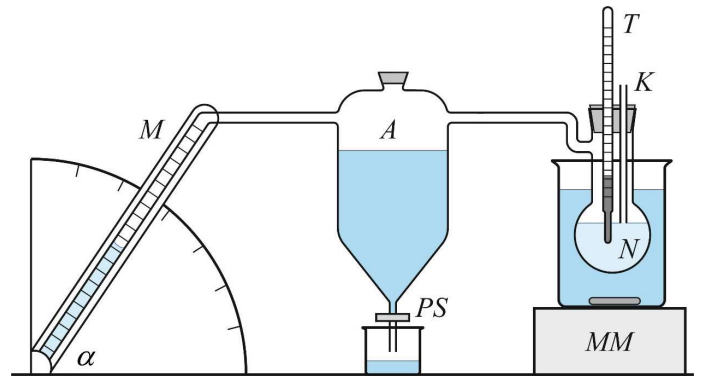
\includegraphics[width=0.75\linewidth]{14 - Studium teplotní závislosti povrchového napětí//Protokol - studium povrchového napětí//img/Aparatura.png}
    \caption{Aparatura pro měření povrchového napětí}
    \label{fig:aparatura-povrchove-napeti}
\end{figure}

% ----------------------------------------------------------------------
%  Výsledky a zpracování měření
% ----------------------------------------------------------------------
\section{Výsledky a zpracování měření}

\subsection{Laboratorní podmínky}

    Měření bylo prováděno za laboratorních podmínek uvedených v tabulce \ref{tab:lab_pod}.

    \begin{table}[h]
        \centering
        \begin{tabular}{|c|c|c|} 
        \hline
            t / °C & p / hPa & vlhkost / \%RH  \\ 
        \hline
            24,3(4)   & 983,2(20)   & 38,9(25)            \\
        \hline
        \end{tabular}
        \caption{Laboratorní podmínky}
        \label{tab:lab_pod}
    \end{table}

\subsection{Podnadpis}

    
% ----------------------------------------------------------------------
%  Diskuse výsledků
% ----------------------------------------------------------------------			
\section{Diskuse výsledků}

% ----------------------------------------------------------------------
%  Závěr
% ----------------------------------------------------------------------
\section{Závěr}
